Dentro del \'atomo podemos distinguir tres componentes: el n\'ucleo at\'omico, los electrones centrales 
y los electrones de valencia (figura \ref{ElectronSeparation}). Los electrones centrales se ubican en las 
capas m\'as cercanas al n\'ucleo  y sus estados  no se ven alterados por la presencia de otros \'atomos, 
es decir se comportan como si fueran inertes. Por el contrario, los electrones de valencia se encuentran 
en las capas m\'as externa del \'atomo y son los responsables del enlace entre los \'atomos. La 
aproximaci\'on del pseudopotencial se basa en estas distinciones entre electrones.

\begin{figure}[H]
    \centering
    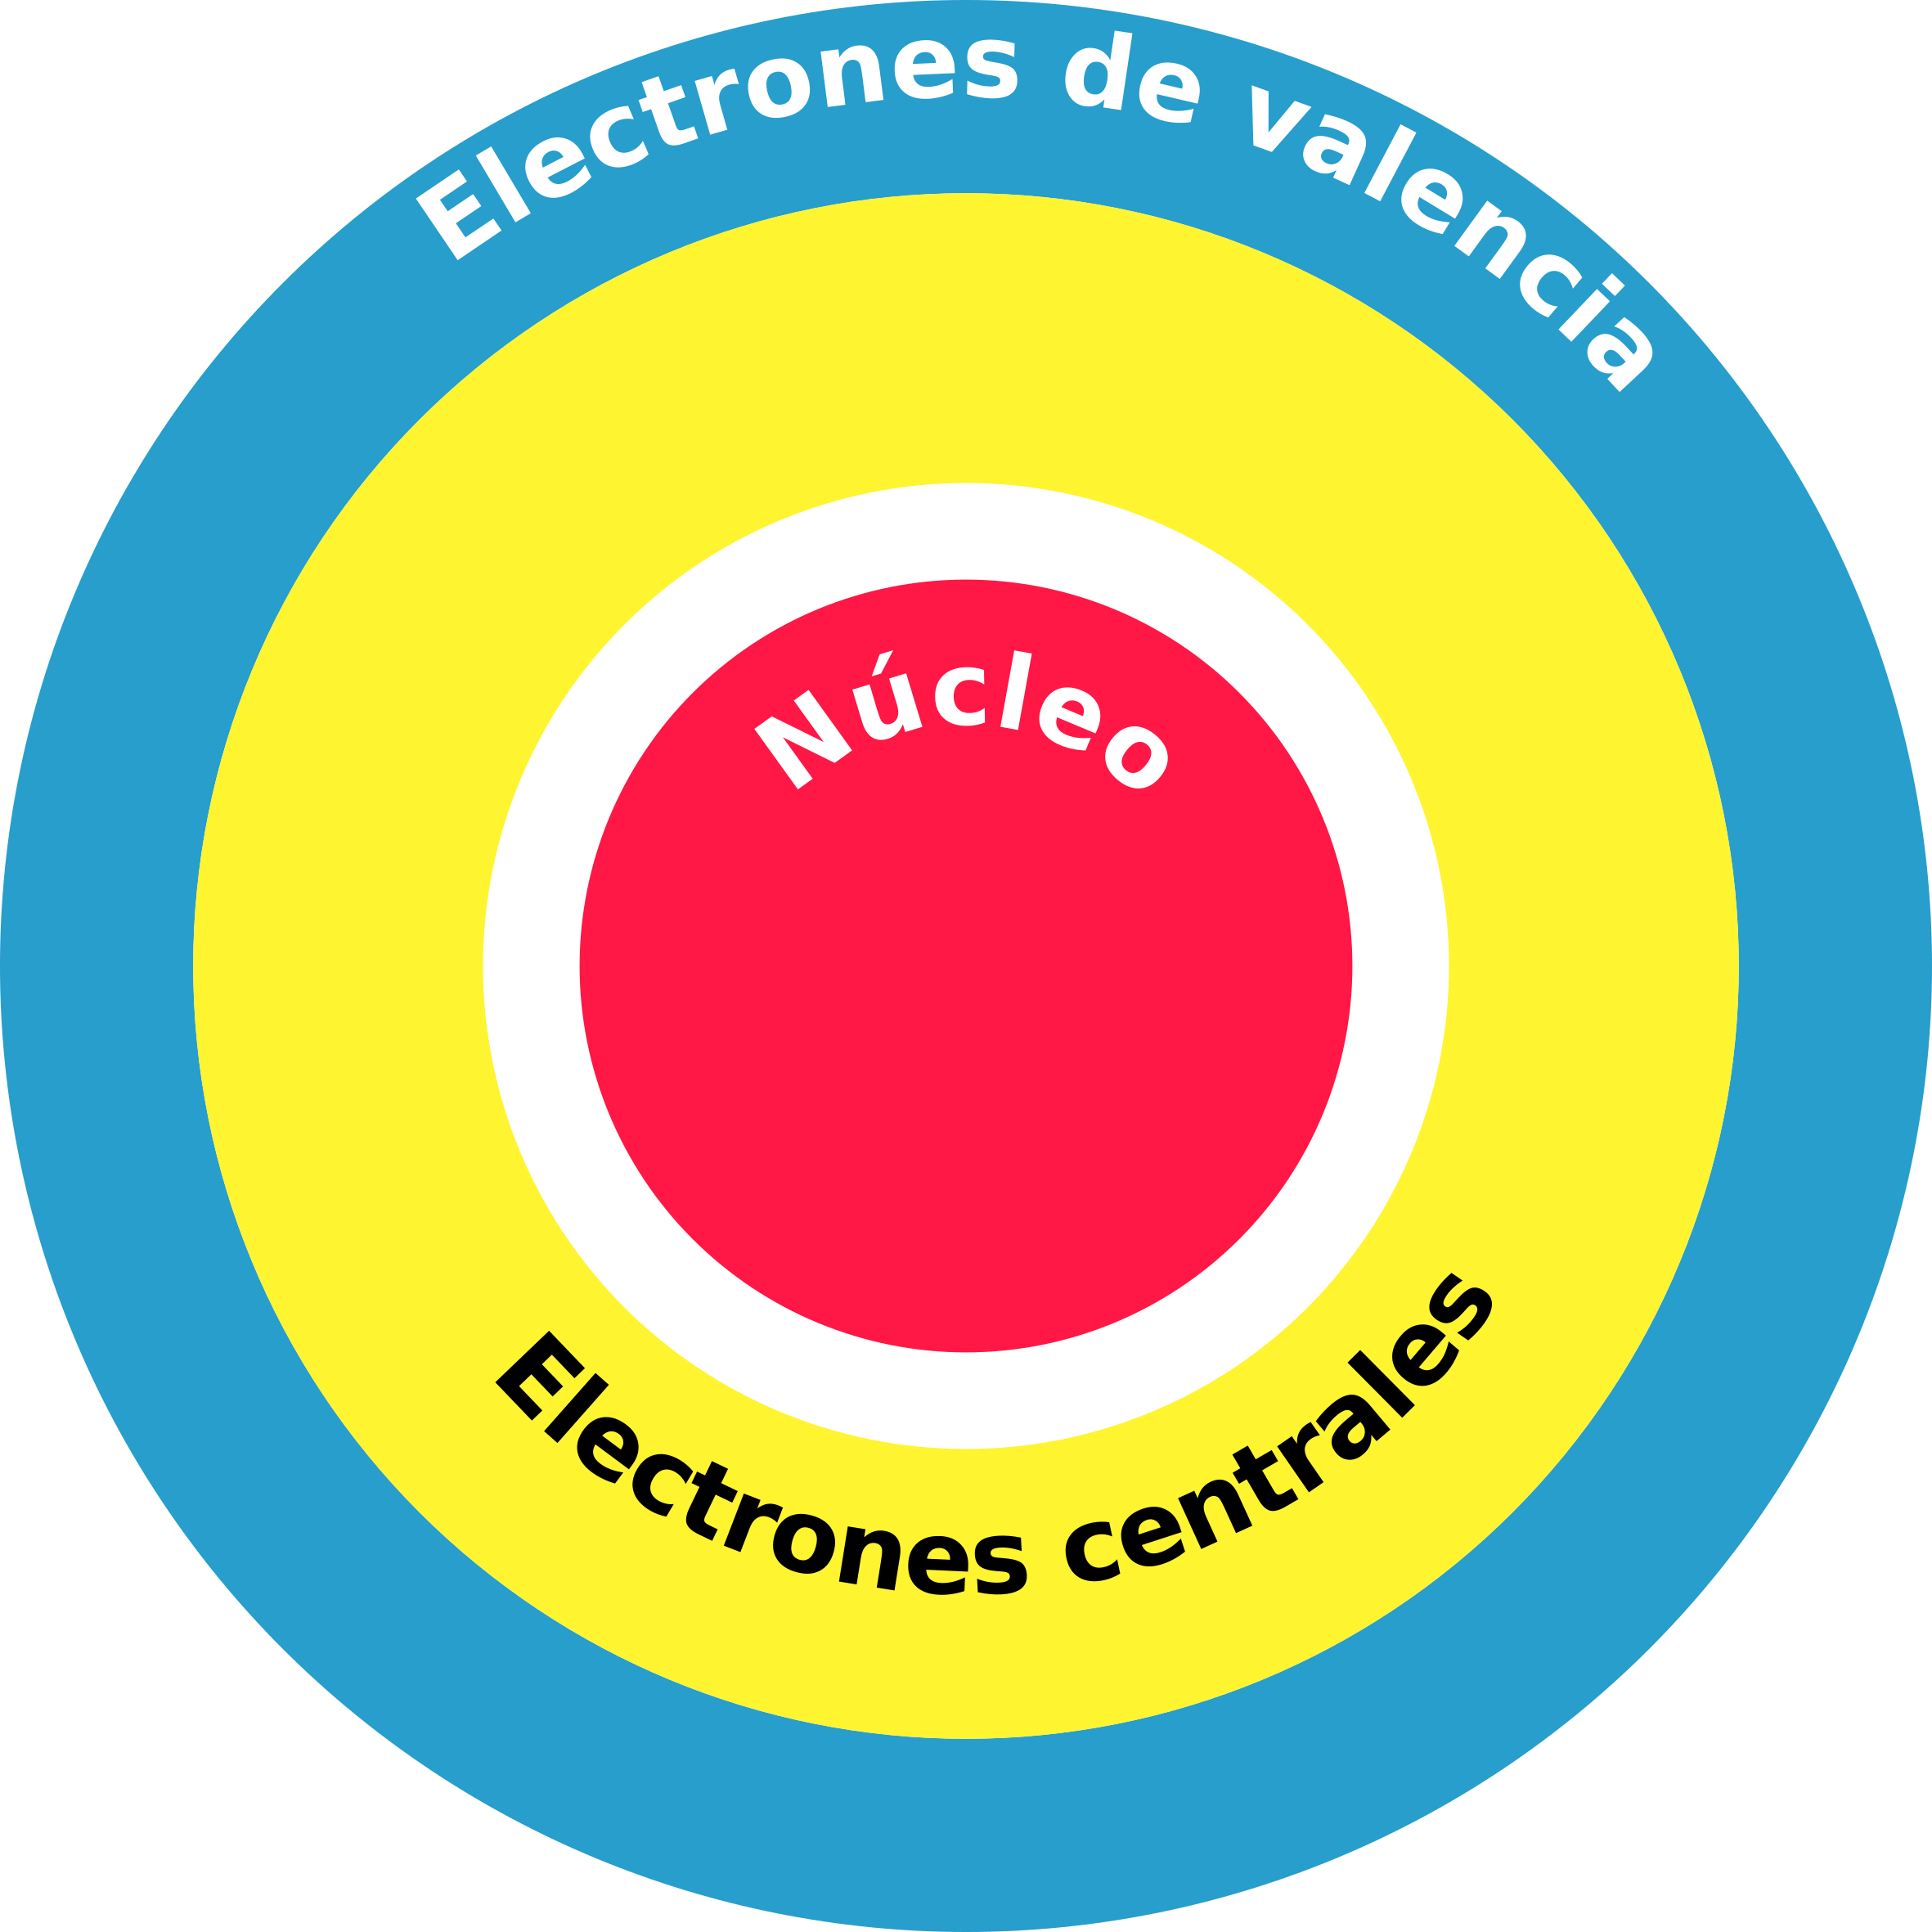
\includegraphics[width=0.3\textwidth]{contenido/marco_teorico/pseudopotencial/img_pseudopotencial/electrons_separation.png}
    \caption[Representaci\'on esquem\'atica de los electrones 
    centrales y de 
    valencia]{Representaci\'on esquem\'atica de los electrones 
    centrales y de 
    valencia.}
    \label{ElectronSeparation}
\end{figure}

\noindent La funci\'on de onda de los electrones de valencia oscila 
r\'apidamente (figura 
\ref{pseudopotential}), cuando 
atraviesa la secci\'on de los electrones centrales dado que estos 
deben 
mantenerse ortogonales entre ellos y hace muy dif\'icil su soluci\'on 
num\'erica. 

\begin{figure}[H]
    \centering
    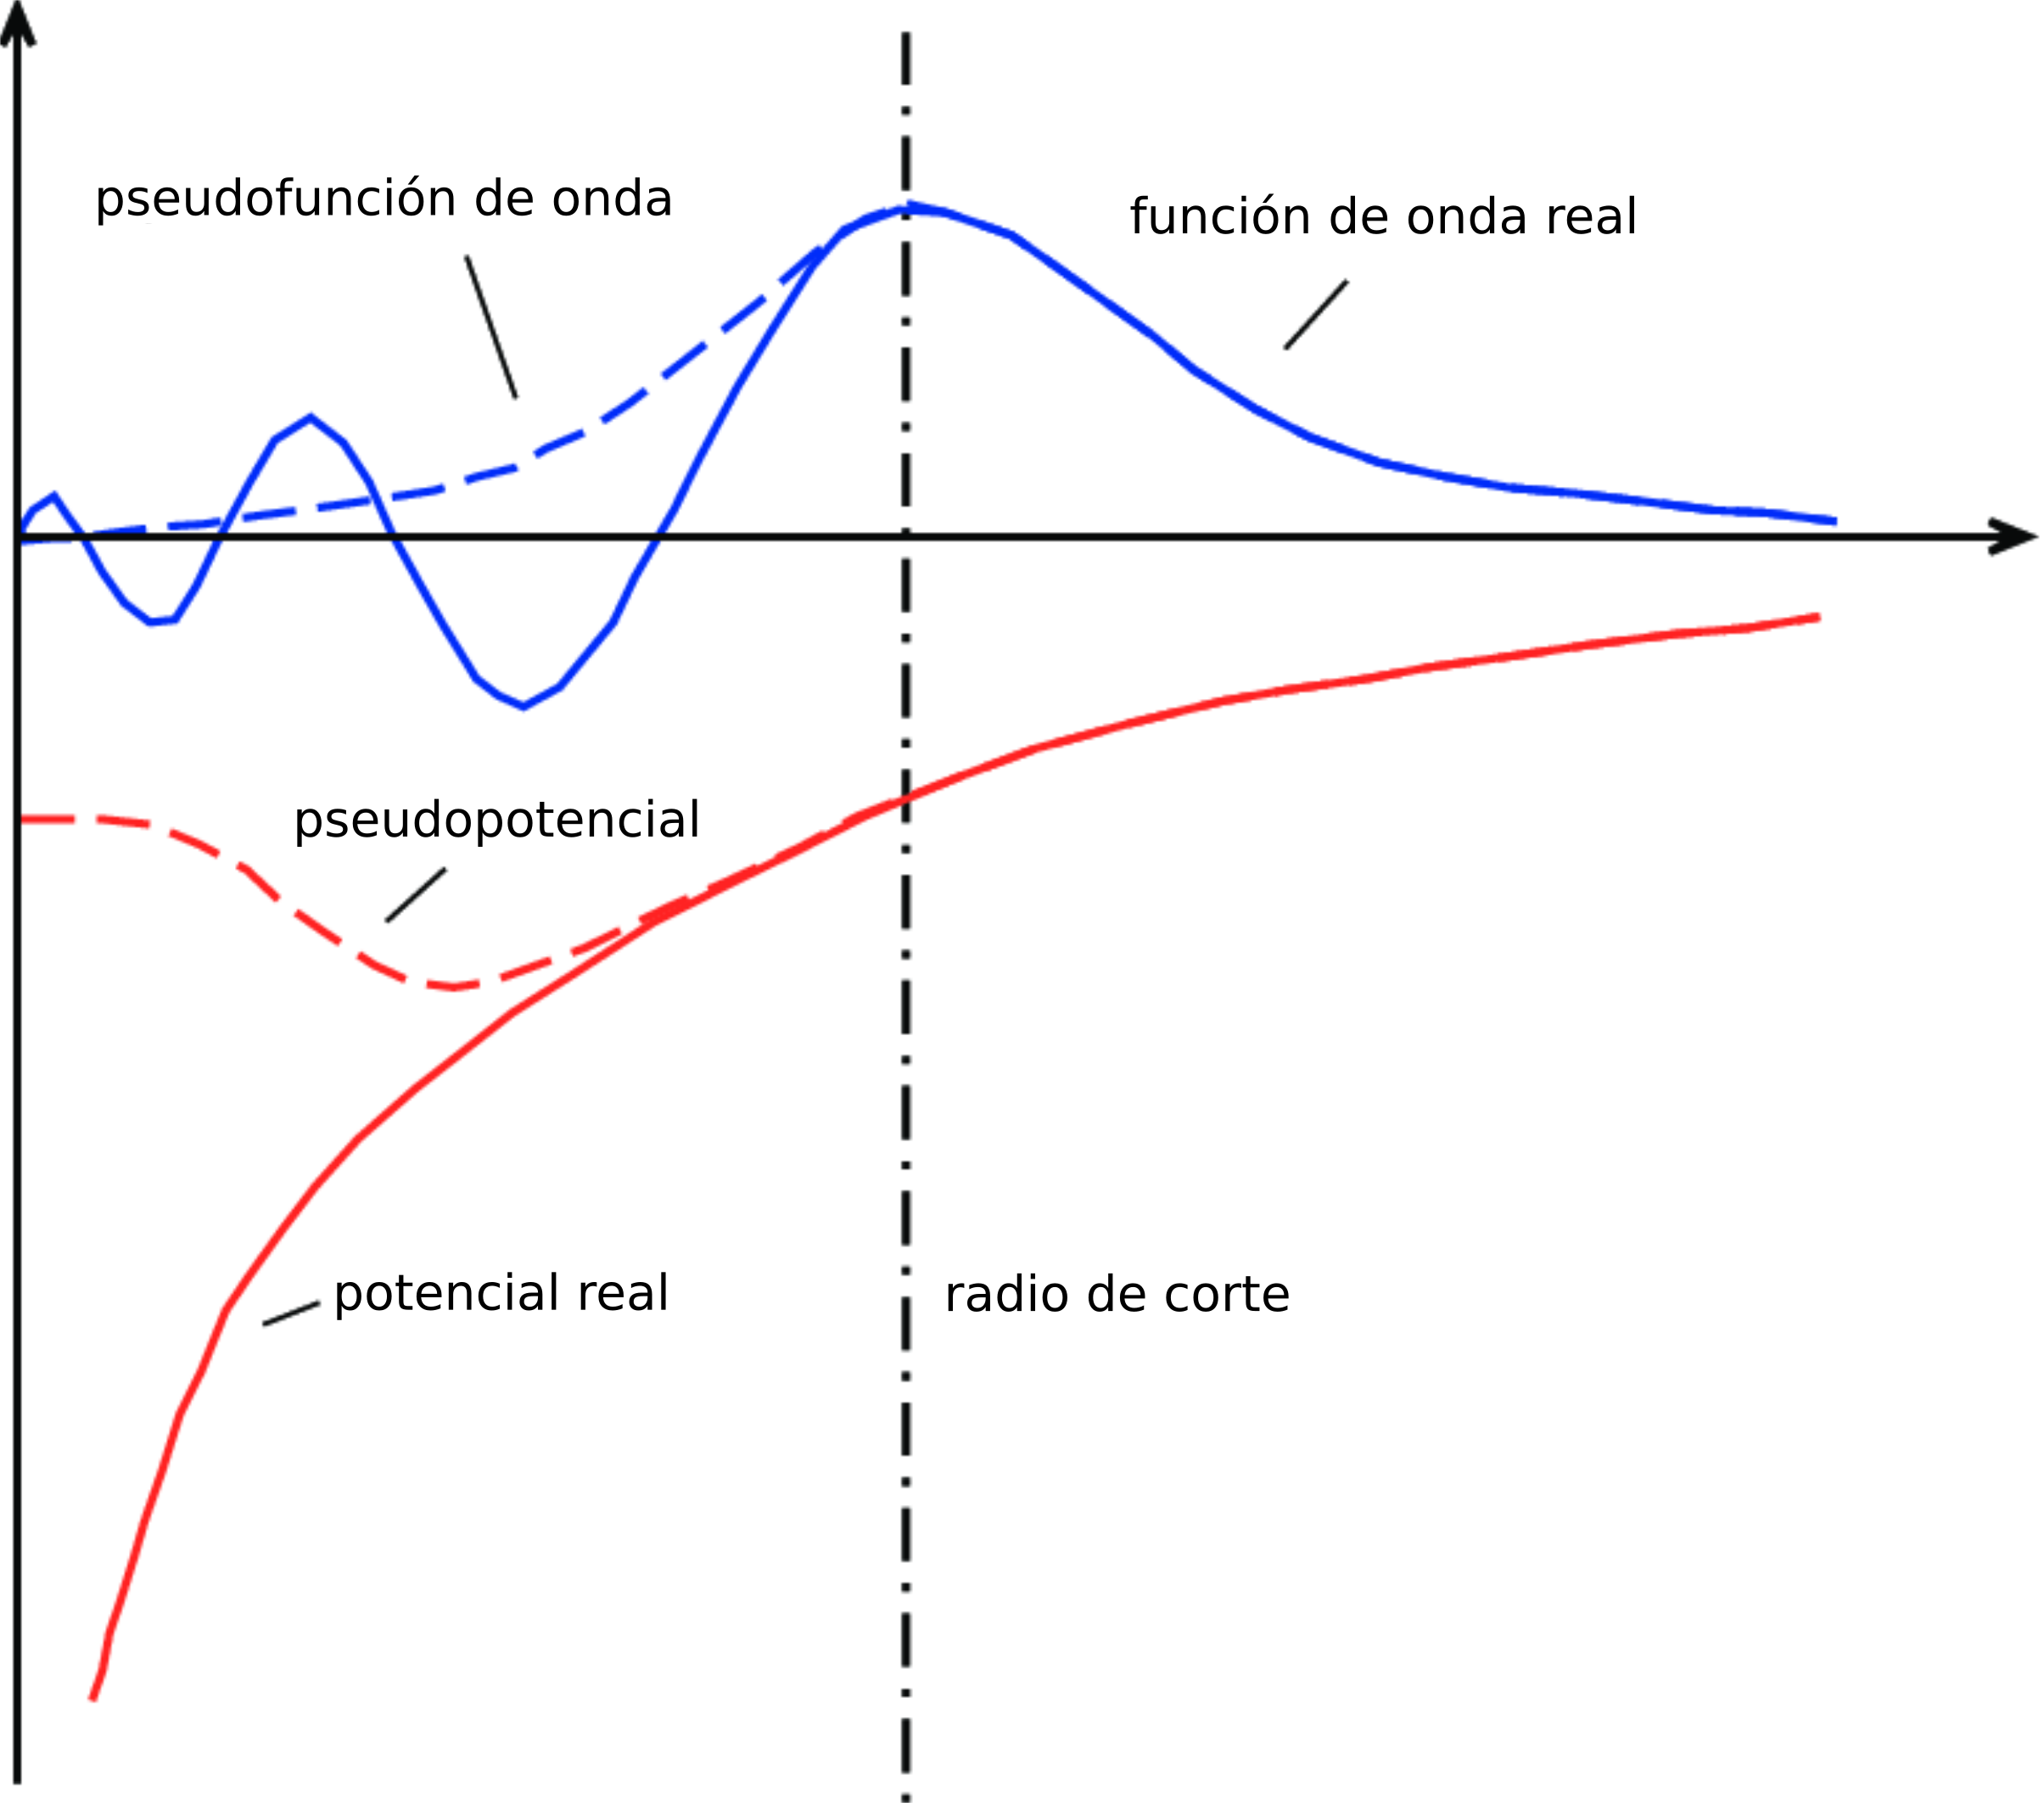
\includegraphics[width=0.4\textwidth]{contenido/marco_teorico/pseudopotencial/img_pseudopotencial/pseudopotential.png}
    \caption[Representaci\'on esquem\'atica del potencial real y del 
    pseudopotencial]{Representaci\'on esquem\'atica del potencial real y del 
    pseudopotencial.}
    \label{pseudopotential}
\end{figure}

\noindent La aproximaci\'on de los pseudopotenciales, reemplaza estas funciones 
de 
valencia por pseudofunciones de valencia que desempe\~nan el mismo rol 
que las 
originales pero evitando el comportamiento nodal cerca del n\'ucleo. 
Esto se 
logra considerando un pseudopotencial m\'as suave que el potencial del 
n\'ucleo 
original (figura \ref{pseudopotential}), debido a que se consideran a 
los 
electrones centrales y al n\'ucleo como una sola entidad que da origen 
al 
pseudopotencial (figura \ref{ElectronUnion}).

\begin{figure}[H]
    \centering
    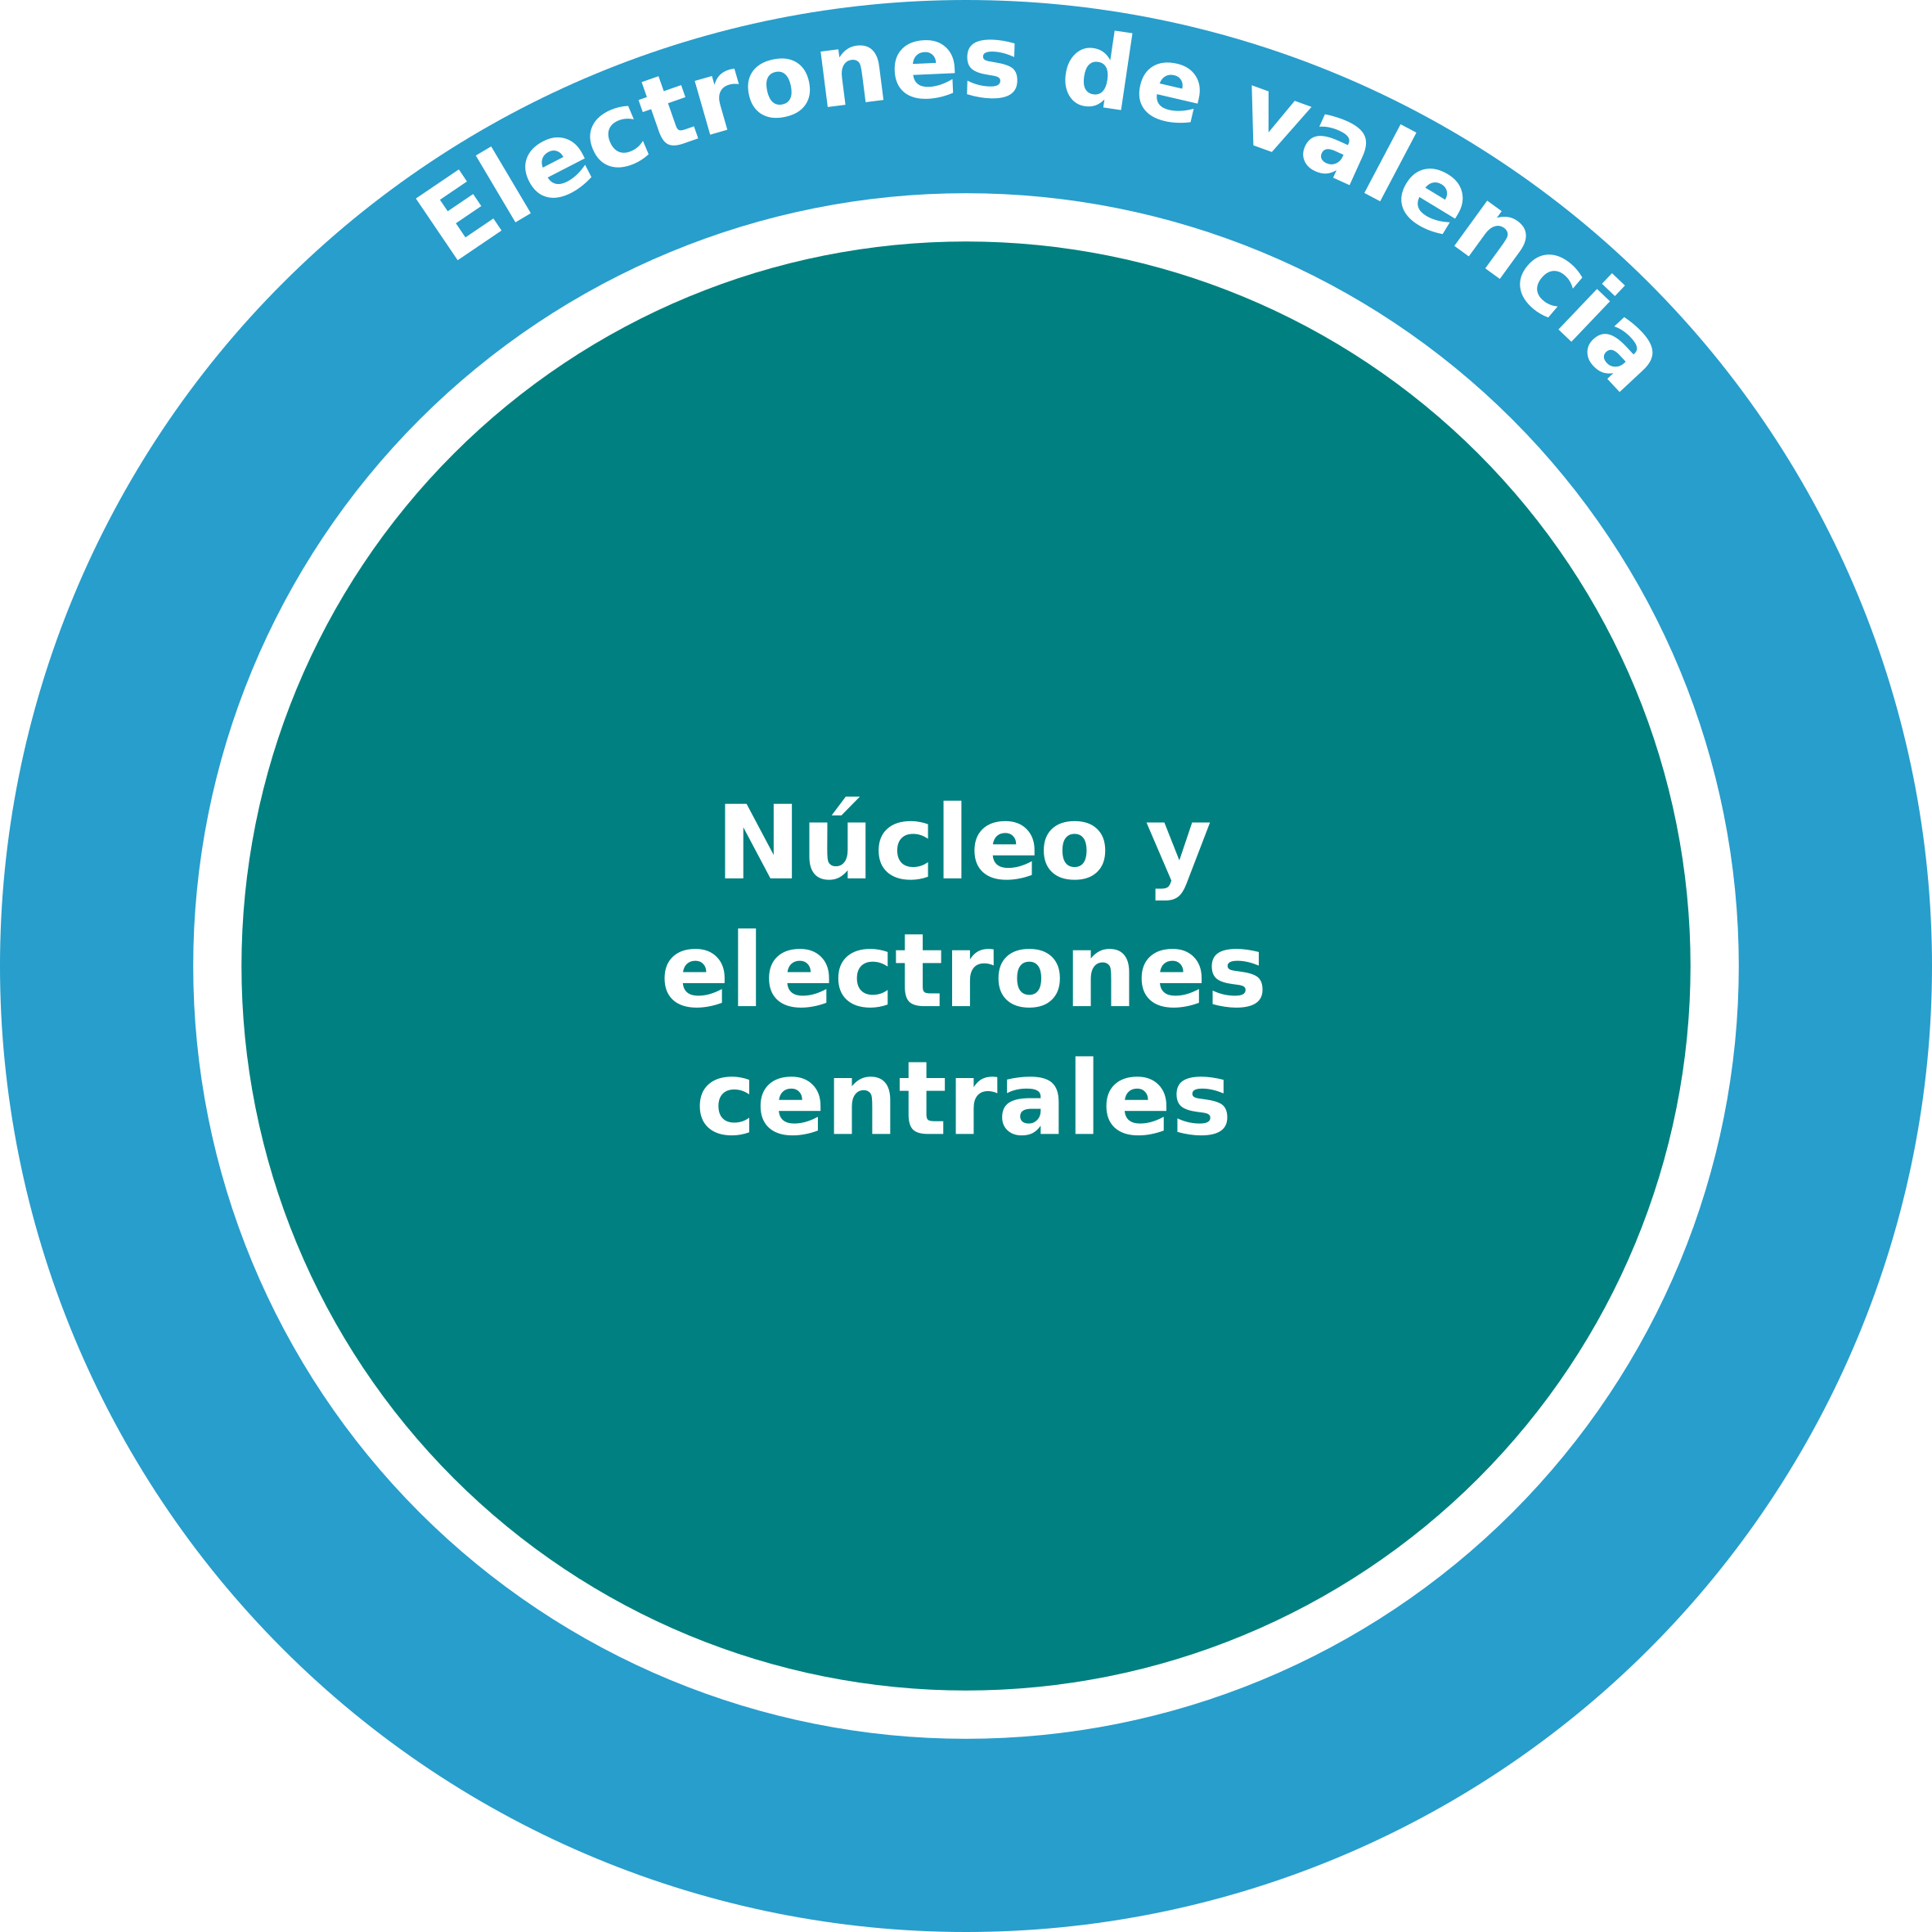
\includegraphics[width=0.3\textwidth]{contenido/marco_teorico/pseudopotencial/img_pseudopotencial/ElectronUnion.png}
    \caption[Representaci\'on esquem\'atica de la aproximaci\'on del 
    n\'ucleo 
    con los electrones centrales]{Representaci\'on esquem\'atica de la 
    aproximaci\'on del 
    n\'ucleo 
    con los electrones centrales.}
    \label{ElectronUnion}
\end{figure}

\noindent Las propiedades de dispersi\'on de cualquier pseudopotencial deben 
ser 
id\'enticas a las propiedades de dispersi\'on del potencial i\'onico 
real. Esto 
es necesario para que el pseudopotencial sea considerado \'util, adem\'as el 
pseudopotencial debe ser transferible es decir que debe ser valido para 
cualquier 
estructura cristalina o s\'olido en el que sea introducido el \'atomo al 
que 
pertenece el pseudopotencial.